\documentclass[11pt]{article}
\usepackage[margin=1in]{geometry}
\usepackage{amsmath}
\usepackage{amssymb}
\usepackage{graphicx}
\usepackage{booktabs}
\usepackage{hyperref}
\usepackage{xcolor}


\title{Project 2}
\author{Kaitlyn Anderson, Mary Bergemann, Reed Wiseman}
\date{November 20, 2026}

\begin{document}
\sloppy
\maketitle

\paragraph{Lotka-Volterra Equations Part 1}\\
\begin{align*}
    \frac{dx}{dt} &= \alpha x-\beta xy\\
    \frac{dy}{dt} &= -\gamma y+\delta xy
\end{align*}\\
The Lotka-Volterra equations is a set of two differential equations with an ecological basis. These equations describe the relationship between a predator and prey or a parasite and a host. The function assumes four fixed rates represented by alpha, beta, gamma, and delta. These numbers describe the growth rate of prey, the rate at which predators kill prey, the rate predators die, and the rate predator population increases due to the fact they are eating the prey, respectively. 

\paragraph{Rössler Attraction Part 1}
\begin{align*}
    \frac{dx}{dt} &= -y-x\\
    \frac{dy}{dt} &= x+ay\\
    \frac{dz}{dt} &= b +z(x-c)\\
\end{align*}

The Rössler Attractor is a third order ordinary differential equation that is separated out into the three equations seen above. Each parameter (a,b,c) is varied, and each one gives a different result including causing the system to converge towards a fixed point, periodic endpoint, or infinity. This system contains two fixed points, one in the middle that is unstable and settles into a chaotic attractor and one on the outside of the region of the attractor. The trajectory starts with the point in the middle of the attractor and continues along its path until it exits the x-y plane where it approaches the second point. This repeats in cycles and ultimately describes the behavior of a chaotic attractor. 

\paragraph{Lotka-Volterra Equations in VS Code}
\begin{verbatim}
    x, y = sp.symbols("x y")
alpha = 1.0   # prey growth rate
beta = 0.1    # predation rate
gamma = 1.5   # predator death rate
delta = 0.075 # predator reproduction rate

def fLV(t, L):
    x, y = L
    dxdt = alpha*x - beta*x*y
    dydt = delta*x*y - gamma*y
    return [dxdt, dydt]

t_span = (0, 20)
t_eval= np.linspace(0, 20, 1000)
y0 = [20, 5]
 
sol = solve_ivp(fLV, t_span, y0)

plt.figure(figsize=(8,5))
plt.plot(sol.t, sol.y[0], label='Prey')
plt.plot(sol.t, sol.y[1], label='Predator')
plt.xlabel('Time')
plt.ylabel('Population')
plt.title('Lotka-Volterra Model')
plt.legend()
plt.grid(True)
plt.show()
\end{verbatim}

\begin{figure}[h]
    \centering
    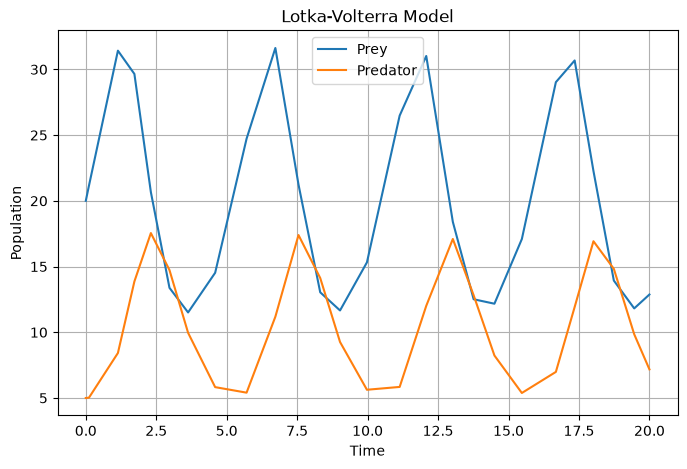
\includegraphics[width=0.5\linewidth]{LV1.png}
    \caption{LV Graph: Parameters \alpha = 1.0, \beta = 0.1, \gamma = 1.5, \delta = 0.075}
    \label{fig:placeholder}
\end{figure}
\begin{figure}[h]
    \centering
    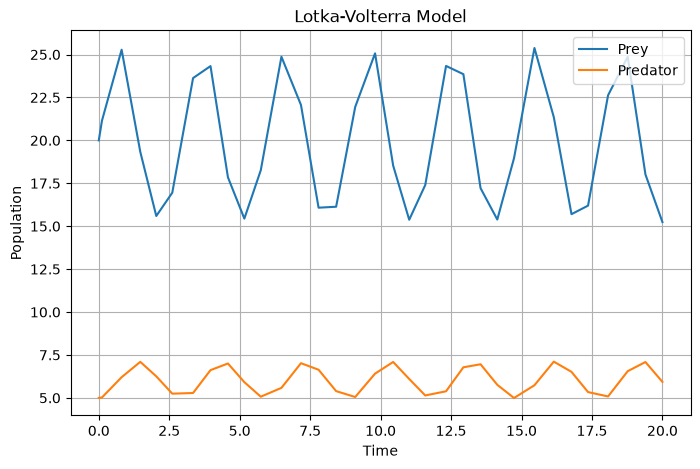
\includegraphics[width=0.5\linewidth]{LV20.png}
    \caption{LV Graph: Parameters \alpha = 3.0, \beta = 0.5, \gamma = 1.5, \delta = 0.075}
    \label{fig:placeholder}
\end{figure}
\begin{figure}[h]
    \centering
    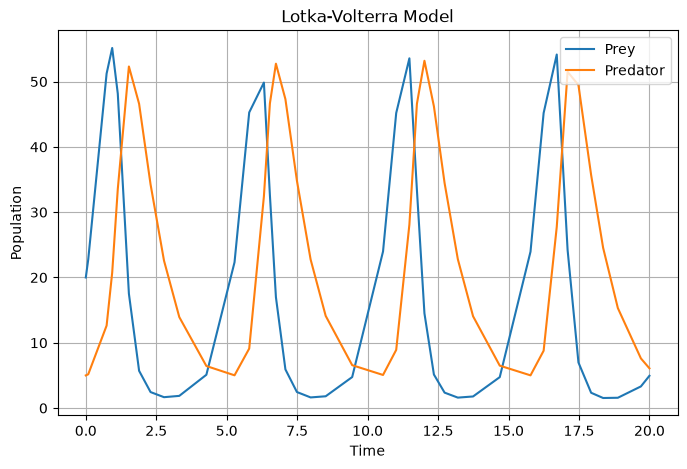
\includegraphics[width=0.5\linewidth]{LV30.png}
    \caption{LV Graph: Parameters \alpha = 2.0, \beta = 0.1, \gamma = 1.0, \delta = 0.065}
    \label{fig:placeholder}
\end{figure}
\clearpage
\paragraph{Rössler Attraction in VS Code}
\begin{verbatim}
    x, y = sp.symbols("x y")
alpha = 1.0   # prey growth rate
beta = 0.1    # predation rate
gamma = 1.5   # predator death rate
delta = 0.075 # predator reproduction rate

def fLV(t, L):
    x, y = L
    dxdt = alpha*x - beta*x*y
    dydt = delta*x*y - gamma*y
    return [dxdt, dydt]

t_span = (0, 20)
t_eval= np.linspace(0, 20, 1000)
y0 = [20, 5]
 
sol = solve_ivp(fLV, t_span, y0)

plt.figure(figsize=(8,5))
plt.plot(sol.t, sol.y[0], label='Prey')
plt.plot(sol.t, sol.y[1], label='Predator')
plt.xlabel('Time')
plt.ylabel('Population')
plt.title('Lotka-Volterra Model')
plt.legend()
plt.grid(True)
plt.show()
\end{verbatim}

\begin{figure}[h]
    \centering
    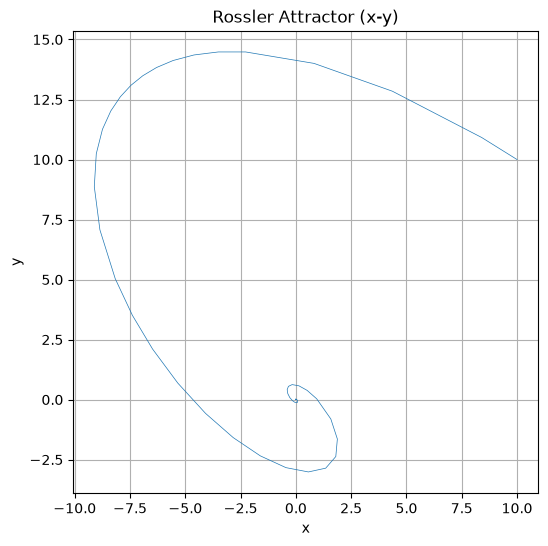
\includegraphics[width=0.5\linewidth]{RA10.png}
    \caption{Rössler Attraction Graph: Parameters a=0.2, b=0.2, c=5.7}
    \label{fig:placeholder}
\end{figure}

\begin{figure}[h]
    \centering
    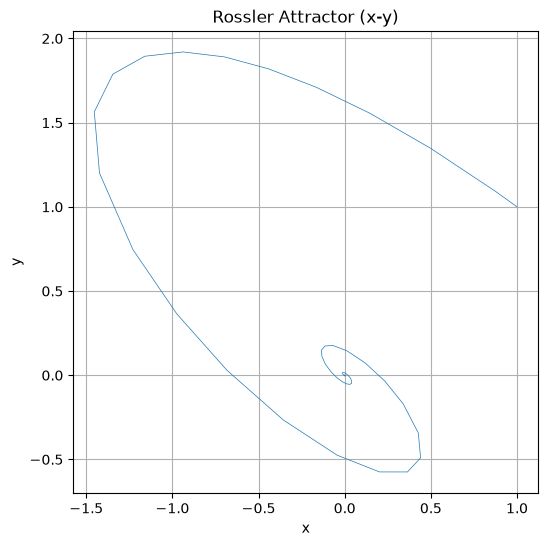
\includegraphics[width=0.5\linewidth]{RA2.png}
    \caption{Rössler Attraction Graph: Parameters a=0.5, b=0.3, c=6.7}
    \label{fig:placeholder}
\end{figure}

\begin{figure}[h]
    \centering
    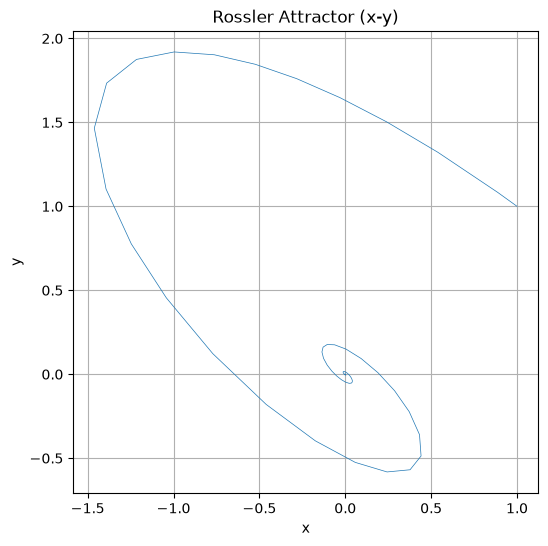
\includegraphics[width=0.5\linewidth]{RA3.png}
    \caption{Rössler Attraction Graph: Parameters a=0.2, b=0.2, c=1.0}
    \label{fig:placeholder}
\end{figure}

\clearpage
\paragraph{Task 3: Numerical Accuracy of the Solver}
\begin{verbatim}
To investigate the accuracy of SciPy's `solve_ivp`, we used the logistic equation \(f'=f(1-f)\), which has a known exact solution. We selected an initial condition of \(f(0)=0.2\) and a final time of \(t=5\).

We calculated numerical solutions using different relative tolerances (`rtol`) ranging from \(10^{-3}\) to \(10^{-10}\), while keeping the absolute tolerance (`atol`) constant at \(10^{-12}\). We then compared each numerical solution with the exact solution at \(t=5\) to calculate its absolute error.

The results show that **decreasing the relative tolerance generally decreases the numerical error**, producing a more accurate approximation. However, smaller tolerances require the solver to take more steps, increasing computational effort.

import numpy as np
import matplotlib.pyplot as plt
from scipy.integrate import solve_ivp

# Implementing logistic differential equation
def logistic(t, f):
    return f * (1 - f)

# Implimenting known exact solution equation
def exact(t, f0):
    return 1 / (1 + ((1 - f0) / f0) * np.exp(-t))

# Defining initial conditions
f0 = 0.2
t_span = (0, 5)

# Generates 8 log values evenly spaced between 10^{-3} and 10^{-10}
rtol_values = np.logspace(-3, -10, 8)

# Generates an empty list
errors = []

# Creates a for loop
for rtol in rtol_values:

    # function for generating a solution using solve_ivp
    # logistic is the function for the Logistic Equation
    # t_span is the time interval from 0 to 5
    # [f0] is the initial population, which we defined as being = 0.2
    # rtol determines how precise the calculated values must be
    # atol is a fixed level of absolute tolerance which we can compare with the changing values of rtol
    sol = solve_ivp(logistic, t_span, [f0], rtol=rtol, atol=1e-12)

    # Calculates the solution using solve_ivp at t = 5
    numerical = sol.y[0, -1]

    # Calculates the solution using the manually derived exact solution formula at t = 5
    actual = exact(5, f0)

    # Calculates absolute error
    error = abs(numerical - actual)

    # Appends each absolute error value to a list
    errors.append(error)

    # Prints each rtol value with its corresponding absolute error value
    print(f"rtol = {rtol:.0e}, Error = {error:.3e}")

rtol = 1e-03, Error = 6.519e-05
rtol = 1e-04, Error = 4.805e-06
rtol = 1e-05, Error = 1.207e-07
rtol = 1e-06, Error = 4.919e-08
rtol = 1e-07, Error = 8.717e-09
rtol = 1e-08, Error = 1.210e-09
rtol = 1e-09, Error = 1.439e-10
rtol = 1e-10, Error = 1.576e-11

# Creating log-log graph for each absolute error value at each rtol value
plt.figure(figsize=(8, 5))

plt.loglog(rtol_values, errors, marker='o')

plt.xlabel('Relative Tolerance (rtol)')
plt.ylabel('Absolute Error')
plt.title('Solver Accuracy vs Relative Tolerance')

plt.grid(True, which='both')
plt.show()
\end{verbatim}

\begin{figure}[h]
    \centering
    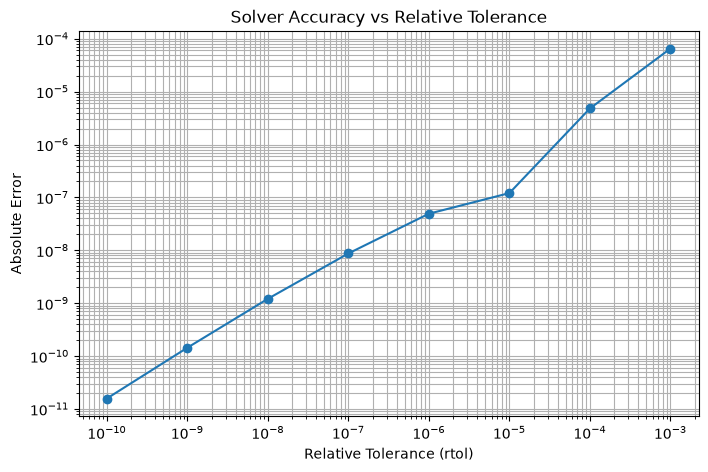
\includegraphics[width=0.5\linewidth]{output.png}
    \caption{Solver Accuracy Vs Relative Tolerance: Parameters $f_0$=0.2, t=(0, 5)}
    \label{fig:placeholder}
\end{figure}

\clearpage
\paragraph{References}-\\
\begin{itemize}
    \item Letellier, Christophe, and Otto E. Rossler. “Rossler Attractor.” Scholarpedia, 3 Oct. 2006, \url{scholarpedia.org/article/R%C3%B6ssler_attractor.}
    \item Wikimedia Foundation. (2026, September 14). List of nonlinear ordinary differential equations. Wikipedia. \url{https://en.wikipedia.org/wiki/List_of_nonlinear_ordinary_differential_equations}
    \item Weisstein, Eric W. "Lotka-Volterra Equations." From MathWorld--A Wolfram Resource. \url{https://mathworld.wolfram.com/Lotka-VolterraEquations.html}
\end{itemize}


\end{document}
